The research plan of this study will follow the work of Peffers et al. described in Section \ref{sec:disMethodology}.

\subsection{Identify, define, and motivate the focal problem}

Our university industry partner has a core service that is pre-employment assessments.
Currently they offer third party organisations an efficient means to bring
candidates on-board which can involve interview(s), medical questionnaires and medical
assessments. Through experience they have realised that sometimes a candidate that appears
perfect for a role fails at the last hurdle of the selection process, being a medical assessment.
It is this late assessment failure that brings rise to the core problem of this research. \textit{How can
    a potential candidate be assessed on some medical criteria without involving an actual medical
    assessment?} A curious reader may wonder why the assessment occurs so late in the process?
This is because the selection process
starts with many multiples of the final number of candidates actually being assessed and so would be prohibitively expensive
to offer the assessments any earlier.


\subsection{Define objectives that a solution (possibly partial) to the focal problem must achieve}

In order to address the focal problem any potential solution should garner useful information from the candidate's answers
to a preselection questionnaire that they are required to complete. The questions contained
within any such questionnaire should take into account the specific role for which the candidate is applying
and any typical risks or needs that are associated with that role.

\subsection{Design and develop the artefact}

Being able to definitively label a role or job title is critical to the operation of any system being developed.
For instance a bus driver could also be referred to as a bus operator or omnibus driver and so a standard convention
is required. This convention within Australia and New Zealand is the Australian and New Zealand Standard Classification
of Occupations (ANZSCO). This ANZSCO standard will form the bridge between the description of a role given by
a third party and the definition of the role within the system. This bridge is described in Figure~\ref{fig:anzcoriskprofile}.
Within the bridge exists an ANZSCO semantic search which represents another research opportunity currently being written
within the university. The bridge also contains multiple "risk profile templates" which represent a predefined "risk profile"
enabling third party's to have a building block for their specific role.

\input{fig/Fig_ANZCO_riskprofile}

The artefacts to be developed should be able to categorise candidates for specific roles where each role is
associated with one or more "risk profiles". The purpose of a risk profile is to form the association between
particular job requirements such as "lifting heavy weight from floor to waist" or "sitting for extended periods"
through to the body parts that are affected
due to that requirement, such as back, arm, leg, or shoulder. From these body parts a number of common injuries are linked and from those injuries
ultimately a series of questions are added to the questionnaire for that role. This risk profile association
for an individual role is shown in Figure~\ref{fig:riskprofile}. In this figure we see two job requirements 1 \& 2
that follow the classic association just described whereas job requirement 3 links directly to multiple question groups.
An example of such a requirement would be a bus driver where a particular licence is a requirement which obviously has
no reliance on a particular body part.


% https://tex.stackexchange.com/questions/64836/change-image-size#64843
%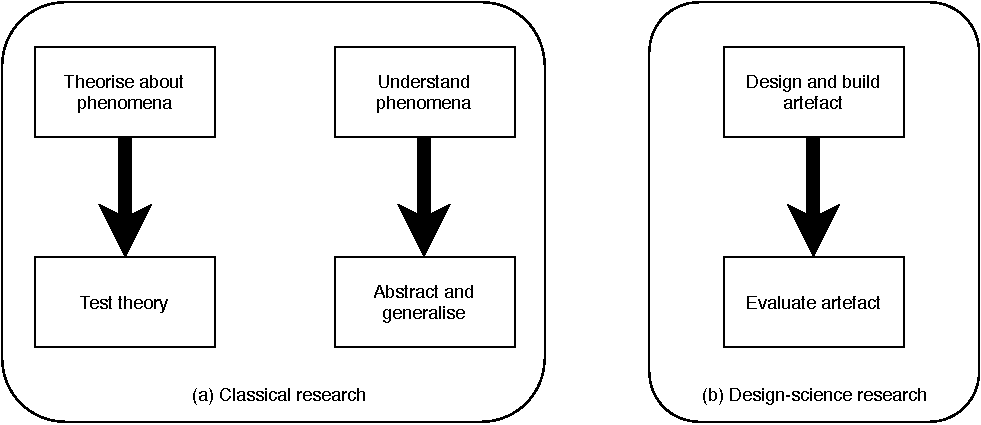
\includegraphics[width=0.9\columnwidth]{TypesOfResearch.pdf}
\begin{figure}[!htb]
    \caption{Risk Profile Setup}
    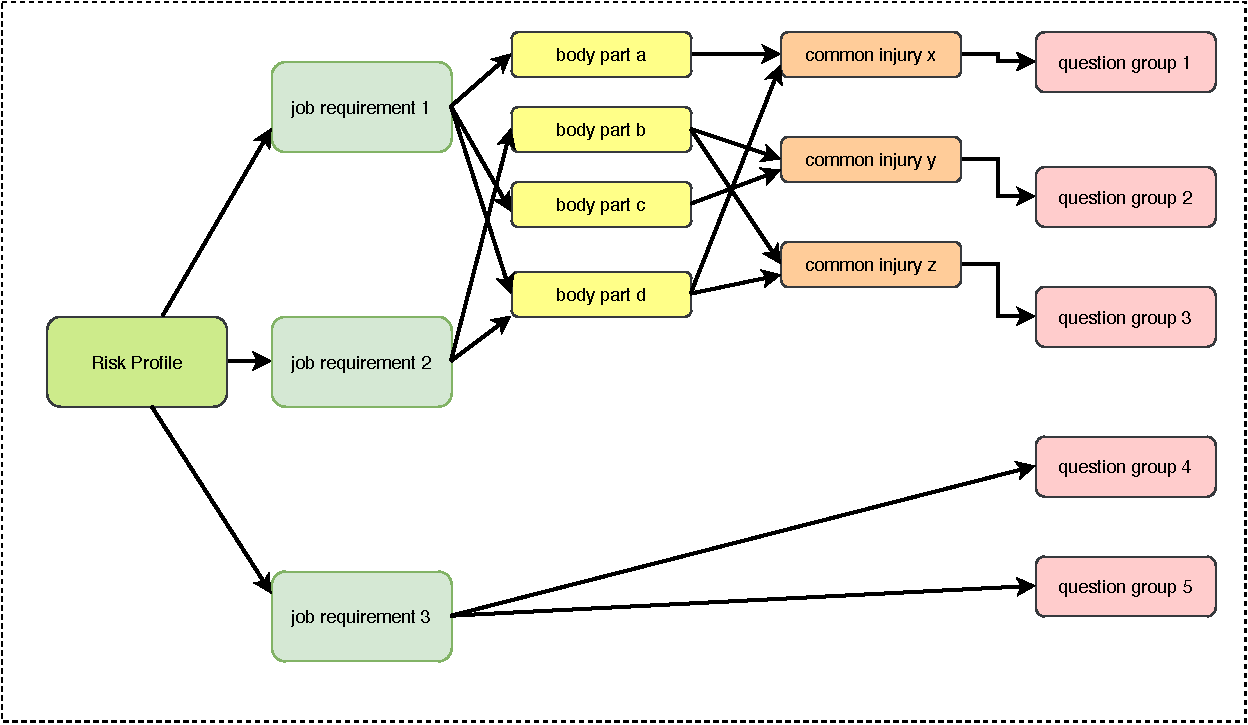
\includegraphics[width=1\columnwidth]{fig/RiskProfile.pdf}
    \label{fig:riskprofile}
\end{figure}


There are a few complications of the questionnaire that a model must adapt to. The first being its hierarchical or cascading
nature which is best described through an example.
A question could be framed asking "have you ever broken your leg?" the answer a candidate gives could be either yes/no.
If the candidate enters "yes" however this could trigger further questions about frequency, time to heal etc. and each
successive answer could themselves create a hierarchical set of questions. The other complication is the fact that answers
to questions can be of various types, for instance a simple quantity like 4, a category like 'male', a list of possible
answers, a ranking like [0-7] or a linguistic ranking like 'tall'.

Initially categorisation of a candidate will involve training an individual classification model for each role from
the answers collected through the associated questionnaire. This classification will be a binary classifier
of "suitable" or "not suitable". It is envisaged that some fuzzy categorisation of the candidate will also be
possible which will allow for a human to override a decision on the candidate who is borderline. The opportunity
to use some form of transfer or cluster learning would remove the need to train all roles separately but the initial
design will not cater for this scenario.


\subsection{Demonstrate the artefact can be used to help solve the focal problem}

Figure~\ref{fig:specificjobrequirement} demonstrates a more specific job requirement for lifting heavy weights from floor
to waist. It has been partially completed for the purpose of explanation only and does not represent a genuine scenario.
Of particular note are the edges for heavy weight,
hip and flexor. It is on these edges that properties will initially be attached such as the value for the actual weight
considered "heavy" by an expert in the field. As our classifier begins to acquire data it is these properties that will
dynamically be altered in order to solve our core problem of classifying a candidate. An added bonus of the classifier
will be the ability to suggest alternate candidate roles to an unsuccessful candidate that they may be suitable for.

% https://tex.stackexchange.com/questions/64836/change-image-size#64843
%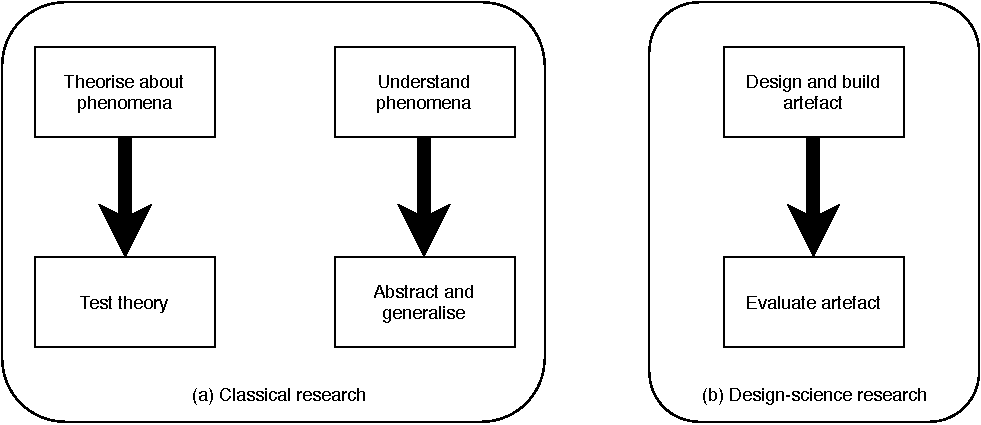
\includegraphics[width=0.9\columnwidth]{TypesOfResearch.pdf}
\begin{figure}[!htb]
    \caption{Specific Job Requirement}
    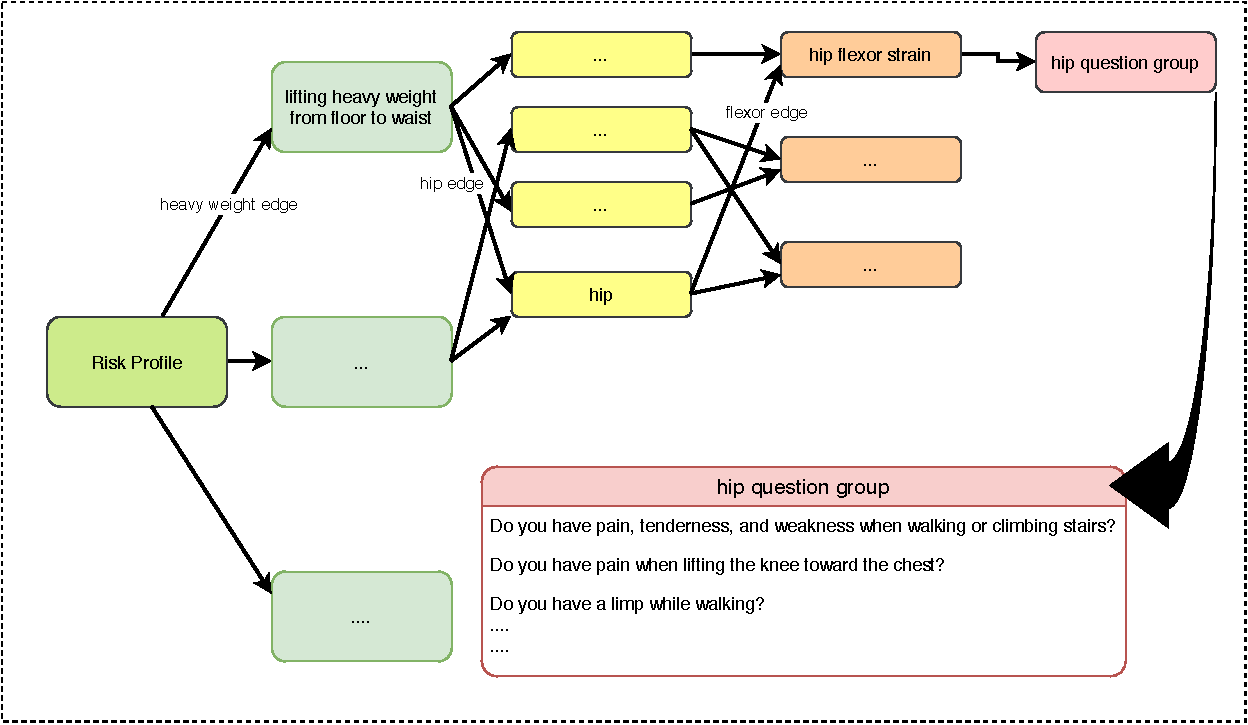
\includegraphics[width=1\columnwidth]{fig/SpecificJobRequirement.pdf}
    \label{fig:specificjobrequirement}
\end{figure}



\subsection{Evaluate how well the artefact solves the focal problem}
\subsection{Communicate the outcomes of the research}


Amongst the outcomes of this research will be the development of a number of novel algorithms to be incorporated into a commercial software product. It is the algorithms that are developed during the design phase that will satisfy the artefact requirement of DSR. The stakeholder community will initially involve the industry partner of the university but will ultimately be useful to anyone dealing with the problem of classifying the answers to closed survey/questionnaire data.



